\documentclass[tikz, crop, border = {2pt 2pt 2pt 2pt}]{standalone}

\usepackage{concmath-otf}
\usetikzlibrary{decorations.pathreplacing, calc}
\usetikzlibrary{patterns}

\begin{document}
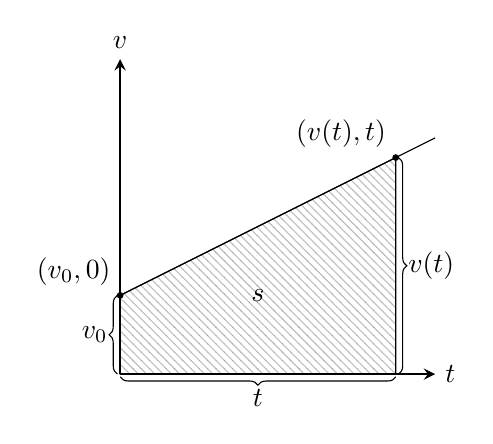
\begin{tikzpicture}
    \draw[thick, -stealth] (0, 0) -- (0, 4) node[above]{$v$};
    \draw[thick, -stealth] (0, 0) -- (4, 0) node[right]{$t$};

    \draw (0, 1) -- (4, 3);
    \draw[dashed] (3.5, 0) -- (3.5, 2.75);

    \coordinate (init) at (0, 1);
    \coordinate (fin) at (3.5, 2.75);

    \draw[decorate, decoration = {brace, amplitude = 3pt, raise = 1pt}] (0, 0) -- (0, 1) node[midway, left = 1pt]{$v_0$};
    \draw[decorate, decoration = {brace, amplitude = 3pt, raise = 1pt, mirror}] (0, 0) -- (3.5, 0) node[midway, below = 2pt]{$t$};
    \draw[decorate, decoration = {brace, amplitude = 3pt, raise = 1pt, mirror}] (3.5, 0) -- ++ (0, 2.75) node[midway, right = 1pt]{$v(t)$};

    \filldraw (init) circle (1pt) node[above left]{$(v_0, 0)$};
    \filldraw (fin) circle (1pt) node[above left]{$(v(t), t)$};

    \filldraw[pattern color = lightgray, pattern = north west lines, blend mode = multiply] (0, 0) -- (init) -- (fin) -- (3.5, 0) -- cycle;
    \node at (1.75, 1){$s$};
\end{tikzpicture}
\end{document}